\documentclass{article}
\usepackage{tikz}
\usetikzlibrary{decorations.pathmorphing} % LATEX and plain TEX when using TikZ
\usetikzlibrary{decorations.pathreplacing} % LATEX and plain TEX when using TikZ
\usetikzlibrary{shapes}
\usetikzlibrary{decorations.markings} % LATEX and plain TEX when using TikZ
\usetikzlibrary{decorations.footprints} % LATEX and plain TEX when using TikZ
\usetikzlibrary{decorations.shapes} % LATEX and plain TEX when using
\usetikzlibrary{decorations.text,math}
\usetikzlibrary{decorations.fractals} % LATEX and plain TEX when using TikZ
\begin{document}
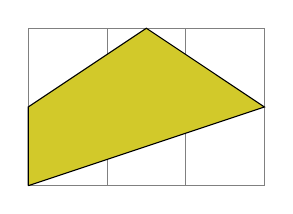
\begin{tikzpicture}[decoration=lineto]
\draw [help lines] grid (3,2);
\draw [decorate,fill=yellow!80!black]
(0,0) -- (3,1) arc (0:180:1.5 and 1) -- cycle;
\end{tikzpicture}
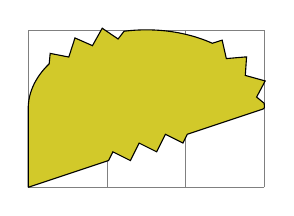
\begin{tikzpicture}[decoration={straight zigzag,meta-segment length=1.1cm}]
\draw [help lines] grid (3,2);
\draw [decorate,fill=yellow!80!black]
(0,0) -- (3,1) arc (0:180:1.5 and 1) -- cycle;
\end{tikzpicture}
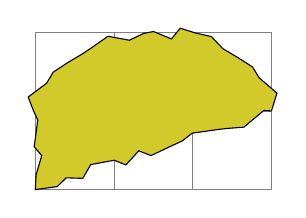
\begin{tikzpicture}
[decoration={random steps,segment length=2mm}]
\draw [help lines] grid (3,2);
\draw [decorate,fill=yellow!80!black]
(0,0) -- (3,1) arc (0:180:1.5 and 1) -- cycle;
\end{tikzpicture}
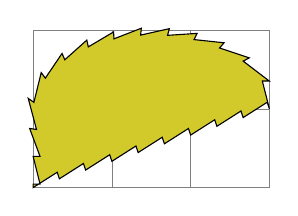
\begin{tikzpicture}[decoration=saw]
\draw [help lines] grid (3,2);
\draw [decorate,fill=yellow!80!black]
(0,0) -- (3,1) arc (0:180:1.5 and 1) -- cycle;
\end{tikzpicture}
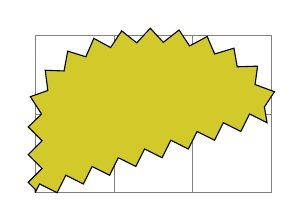
\begin{tikzpicture}[decoration=zigzag]
\draw [help lines] grid (3,2);
\draw [decorate,fill=yellow!80!black]
(0,0) -- (3,1) arc (0:180:1.5 and 1) -- cycle;
\end{tikzpicture}
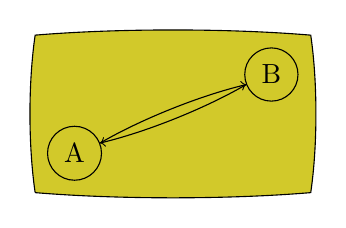
\begin{tikzpicture}[decoration={bent,aspect=.3}]
\draw [decorate,fill=yellow!80!black] (0,0) rectangle (3.5,2);
\node[circle,draw] (A) at (.5,.5) {A};
\node[circle,draw] (B) at (3,1.5) {B};
\draw[->,decorate] (A) -- (B);
\draw[->,decorate] (B) -- (A);
\end{tikzpicture}
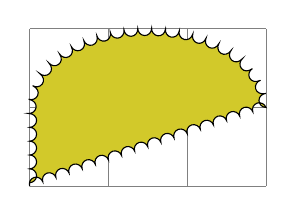
\begin{tikzpicture}[decoration=bumps]
\draw [help lines] grid (3,2);
\draw [decorate,fill=yellow!80!black]
(0,0) -- (3,1) arc (0:180:1.5 and 1) -- cycle;
\end{tikzpicture}
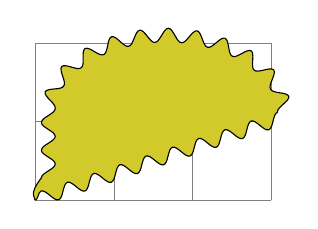
\begin{tikzpicture}[decoration=snake]
\draw [help lines] grid (3,2);
\draw [decorate,fill=yellow!80!black]
(0,0) -- (3,1) arc (0:180:1.5 and 1) -- cycle;
\end{tikzpicture}
%%%%
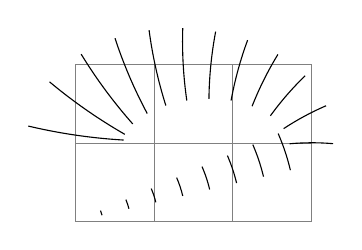
\begin{tikzpicture}[decoration={expanding waves,angle=5}]
\draw [help lines] grid (3,2);
\draw [decorate] (0,0) -- (3,1) arc (0:180:1.5 and 1);
\end{tikzpicture}
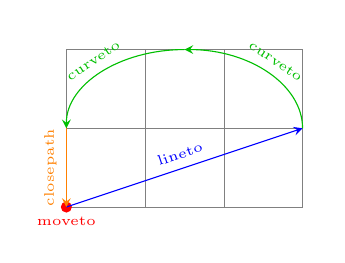
\begin{tikzpicture}[>=stealth, every node/.style={midway, sloped, font=\tiny},
decoration={show path construction,
moveto code={
\fill [red] (\tikzinputsegmentfirst) circle (2pt)
node [fill=none, below] {moveto};},
lineto code={
\draw [blue,->] (\tikzinputsegmentfirst) -- (\tikzinputsegmentlast)
node [above] {lineto};
},
curveto code={
\draw [green!75!black,->] (\tikzinputsegmentfirst) .. controls
(\tikzinputsegmentsupporta) and (\tikzinputsegmentsupportb)
..(\tikzinputsegmentlast) node [above] {curveto};
},
closepath code={
\draw [orange,->] (\tikzinputsegmentfirst) -- (\tikzinputsegmentlast)
node [above] {closepath};}
}]
\draw [help lines] grid (3,2);
\path [decorate] (0,0) -- (3,1) arc (0:180:1.5 and 1) -- cycle;
\end{tikzpicture}

\tikzset{
show curve controls/.style={
decoration={
show path construction,
curveto code={
\draw [blue, dashed]
(\tikzinputsegmentfirst) -- (\tikzinputsegmentsupporta)
node [at end, cross out, draw, solid, red, inner sep=2pt]{};
\draw [blue, dashed]
(\tikzinputsegmentsupportb) -- (\tikzinputsegmentlast)
node [at start, cross out, draw, solid, red, inner sep=2pt]{};
}
},decorate
}
}
\tikzpicture
\draw [postaction=show curve controls, thick]
(0,2) .. controls (2.5,1.5) and (0.5,0.5) .. (3,0);
\endtikzpicture
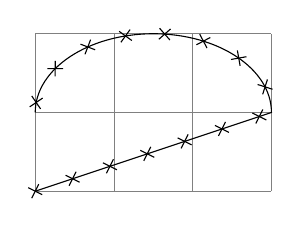
\begin{tikzpicture}[decoration={
markings,% switch on markings
mark=% actually add a mark
between positions 0 and 1 step 5mm
with
{
\draw (-2pt,-2pt) -- (2pt,2pt);
\draw (2pt,-2pt) -- (-2pt,2pt);
}
}]
\draw [help lines] grid (3,2);
\draw [postaction={decorate}] (0,0) -- (3,1) arc (0:180:1.5 and 1);
\end{tikzpicture}
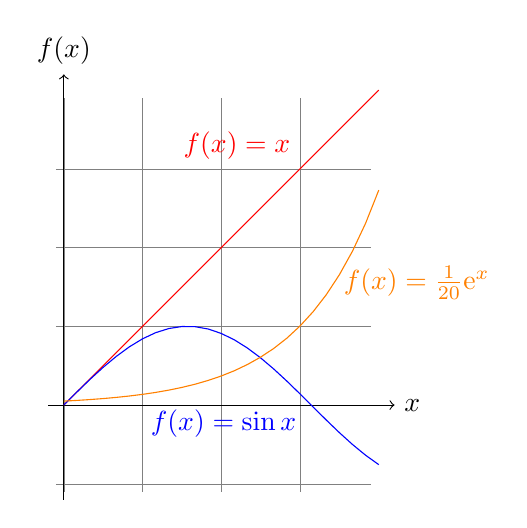
\begin{tikzpicture}[domain=0:4,label/.style={postaction={
decorate,
decoration={
markings,
mark=at position .75 with \node #1;}}}]
\draw[very thin,color=gray] (-0.1,-1.1) grid (3.9,3.9);
\draw[->] (-0.2,0) -- (4.2,0) node[right] {$x$};
\draw[->] (0,-1.2) -- (0,4.2) node[above] {$f(x)$};
\draw[red,label={[above left]{$f(x)=x$}}] plot (\x,\x);
\draw[blue,label={[below left]{$f(x)=\sin x$}}] plot (\x,{sin(\x r)});
\draw[orange,label={[right]{$f(x)= \frac{1}{20} \mathrm e^x$}}] plot (\x,{0.05*exp(\x)});
\end{tikzpicture}
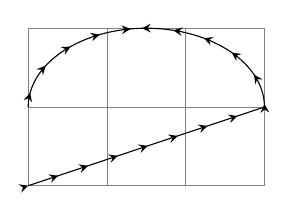
\begin{tikzpicture}[decoration={
markings,% switch on markings
mark=between positions 0 and .75 step 4mm with {\arrow{stealth}},
mark=between positions .75 and 1 step 4mm with {\arrowreversed{stealth}}}
]
\draw [help lines] grid (3,2);
\draw [postaction={decorate}] (0,0) -- (3,1) arc (0:180:1.5 and 1);
\end{tikzpicture}
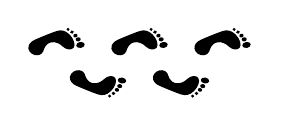
\begin{tikzpicture}[decoration={footprints,foot length=20pt}]
\fill [decorate] (0,0) -- (3,0);
\end{tikzpicture}
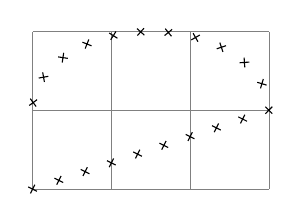
\begin{tikzpicture}[decoration=crosses]
\draw [help lines] grid (3,2);
\draw [decorate] (0,0) -- (3,1) arc (0:180:1.5 and 1);
\end{tikzpicture}
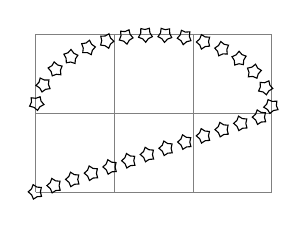
\begin{tikzpicture}[decoration={shape backgrounds,shape=star,shape size=5pt}]
\draw [help lines] grid (3,2);
\draw [decorate] (0,0) -- (3,1) arc (0:180:1.5 and 1);
\end{tikzpicture}
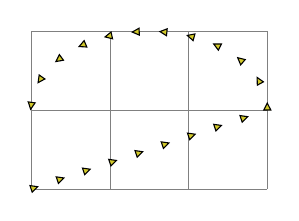
\begin{tikzpicture}[decoration=triangles]
\draw [help lines] grid (3,2);
\draw [decorate,fill=yellow!80!black] (0,0) -- (3,1) arc (0:180:1.5 and 1);
\end{tikzpicture}
\tikzset{paint/.style={ draw=#1!50!black, fill=#1!50 },
decorate with/.style=
{decorate,decoration={shape backgrounds,shape=#1,shape size=2mm}}}
\begin{tikzpicture}
\draw [decorate with=dart, paint=red] (0,1.5) -- (3,1.5);
\draw [decorate with=diamond, paint=green] (0,1) -- (3,1);
\draw [decorate with=rectangle, paint=blue] (0,0.5) -- (3,0.5);
\draw [decorate with=circle, paint=yellow] (0,0) -- (3,0);
\end{tikzpicture}

\bfseries\large
%\catcode `\|12
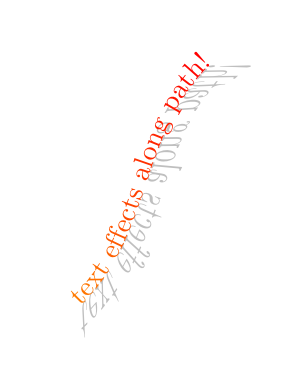
\begin{tikzpicture}[decoration={text effects along path,
                    text={text effects along path!}, text align=center,
                    text effects/.cd,
                    character count=\i, character total=\n,
                    characters={evaluate={\c=\i/\n*100;}, text along path, text=red!\c!orange},
                    character widths={text along path, xslant=0, yscale=1}}]
    \path [postaction={decorate}, preaction={decorate,
                text effects={characters/.append={yscale=-1.5, opacity=0.5,
                text=gray, xslant=(\i/\n-0.5)*3}}}]
        (0,0) .. controls ++(2,1) and ++(-2,-1) .. (3,4);
\end{tikzpicture}

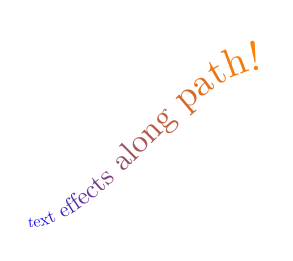
\begin{tikzpicture}[decoration={text effects along path,
text={text effects along path!},
text effects/.cd,
character count=\i, character total=\n,
characters={text along path, evaluate={\c=\i/\n*100;},
text=orange!\c!blue, scale=\i/\n+0.5}}]
\path [decorate]
(0,0) .. controls ++(1,0) and ++(-1,0) .. (3,2);
\end{tikzpicture}

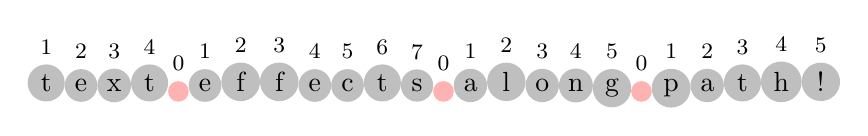
\begin{tikzpicture}[decoration={text effects along path,
text={text effects along path!},
text effects/.cd,
path from text, letter count=\i, every word separator/.style={fill=red!30},
characters={text along path, shape=circle, fill=gray!50}}]
\path [decorate, text effects={characters/.append={label=above:\footnotesize\i}}] (0,0);
\end{tikzpicture}

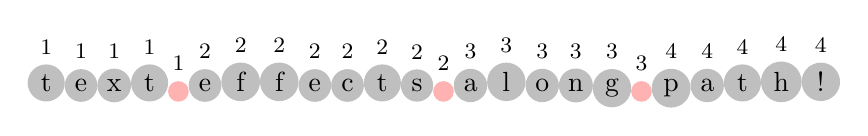
\begin{tikzpicture}[decoration={text effects along path,
text={text effects along path!},
text effects/.cd,
path from text, word count=\i, every word separator/.style={fill=red!30},
characters={text along path, shape=circle, fill=gray!50}}]
\path [decorate, text effects={characters/.append={label=above:\footnotesize\i}}] (0,0);
\end{tikzpicture}


\begin{tikzpicture}[decoration={text effects along path,
text={text effects along path!},
text effects/.cd,
path from text,
character count=\i, character total=\n,
characters={text along path, scale=\i/\n+0.5}}]
\path [decorate] (0,0);
\end{tikzpicture}

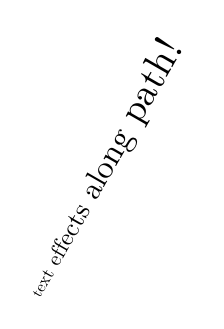
\begin{tikzpicture}[decoration={text effects along path,
text={text effects along path!},
text effects/.cd,
path from text, path from text angle=60,
character count=\i, character total=\n,
characters={text along path, scale=\i/\n+0.5}}]
\path [decorate] (0,0);
\end{tikzpicture}

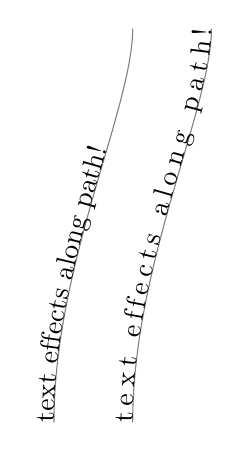
\begin{tikzpicture}[decoration={text effects along path,
text={text effects along path!},
text effects/every character/.style={text along path}}]
\path [draw=gray, postaction={decorate}, rotate=90]
(0,0) .. controls ++(2,0) and ++(-1,0) .. (5,-1);
\path [draw=gray, postaction={decorate}, rotate=90, yshift=-1cm,
text effects={fit text to path}]
(0,0) .. controls ++(2,0) and ++(-1,0) .. (5,-1);
\end{tikzpicture}

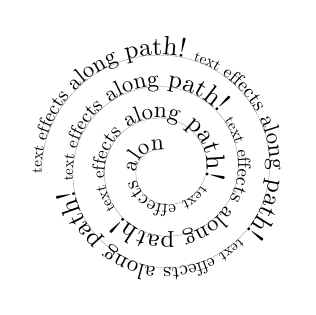
\begin{tikzpicture}[decoration={text effects along path,
text={text effects along path!\ },
text effects/.cd,
repeat text,
character count=\m, character total=\n,
characters={text along path, scale=0.5+\m/\n/2}}]
\path [draw=gray, ultra thin, postaction=decorate]
(180:2) \foreach \a in {0,...,12}{ arc (180-\a*90:90-\a*90:1.5-\a/10) };
\end{tikzpicture}

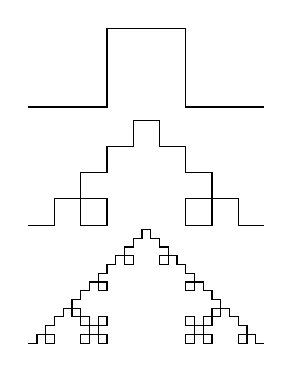
\begin{tikzpicture}[decoration=Koch curve type 1]
\draw decorate{ (0,0) -- (3,0) };
\draw decorate{ decorate{ (0,-1.5) -- (3,-1.5) }};
\draw decorate{ decorate{ decorate{ (0,-3) -- (3,-3) }}};
\end{tikzpicture}

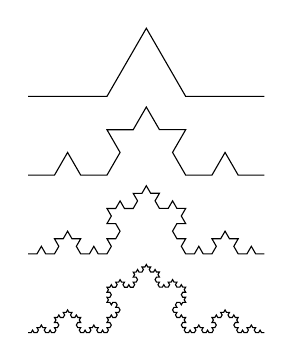
\begin{tikzpicture}[decoration=Koch snowflake]
\draw decorate{ (0,0) -- (3,0) };
\draw decorate{ decorate{ (0,-1) -- (3,-1) }};
\draw decorate{ decorate{ decorate{ (0,-2) -- (3,-2) }}};
\draw decorate{ decorate{ decorate{ decorate{ (0,-3) -- (3,-3) }}}};
\end{tikzpicture}

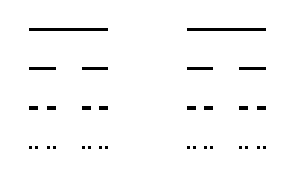
\begin{tikzpicture}[decoration=Cantor set,very thick]
\draw decorate{ (0,0) -- (3,0) };
\draw decorate{ decorate{ (0,-.5) -- (3,-.5) }};
\draw decorate{ decorate{ decorate{ (0,-1) -- (3,-1) }}};
\draw decorate{ decorate{ decorate{ decorate{ (0,-1.5) -- (3,-1.5) }}}};
\end{tikzpicture}
\end{document}